\chapter{Representations for trips over public transportation networks}
\label{sec:newctr}

	After \gls{ctr} was introduced in Chapter~\ref{sec:ctr} as a representation oriented for trips over urban street networks, in this chapter we introduce two alternative representations, called \acrfull{ttctr} and \acrfull{xctr}. These new techniques are expected to be more adequate for trips over public transportation networks, since they make it possible to query about network concepts such as line and schedules, and also use them in order to reduce the size of our structures.
	
	Both \gls{ttctr} and \gls{xctr} are also based on the \gls{csa}  and the \gls{wm}, although they rely on other common structures for a network representation, that do not need to be compact due to their already small size. However, we have found out that while these representations excel at many of our proposed queries related to trip patterns, they could be rather inefficient for other kinds of aggregation queries about the load of a network. For this reason, we have also introduced a complementary \acrfull{tm}, a \gls{sat}-based structure designed to accelerate this second kind of queries.
	
	We have implemented and evaluated our structures, over the current bus network of Madrid, thus analyzing, both theoretically and experimentally, the fitness of each representation for every use case. This chapter starts with a brief description of the scenario where we identify all the elements involved in a public transportation network, and we also identify the most significative queries that should be considered. Then, in Section~\ref{sec:newctr:str}, we present all the structures considered in our proposal. This includes the common structures to manage \mbox{network-related} elements, and the structures \gls{ttctr}, \gls{xctr}, and \gls{tm}. In Section~\ref{sec:newctr:algo}, we show how to support queries. Finally, we analyze them theoretically in Section~\ref{sec:newctr:algo:analysis}, and experimentally in Section~\ref{sec:newctr:exp}, where we measure both the space needs and query performance. Additionally, in Chapter~\ref{sec:gis} we will show how these representations can be integrated into a GIS application, usable for a transportation network administrator.
	
\section{Description}
    \label{sec:newctr:desc}
	While, in theory, we could use the \gls{ctr} (Chapter~\ref{sec:ctr}) to also represent trips over a subway or bus network, such representation would be very redundant. If we defined our \gls{ctr} nodes as stops or stations, making two of them connected if there exists a line or route that stops at each, we would find out that a commuter would board at a stop and follow only one route (line), passing through all its stops consecutively until the alighting stop, either to switch lines or end the trip. Furthermore, a single vehicle (such as a bus or a train) will be shared by several commuters at the same time, thus also producing trips that visit the same nodes at the same times. Because simply listing every node traversed introduces all these kinds of redundancy for public transportation networks, we state that \gls{ctr} is more adequate for urban street networks.
	
	Therefore, in order to better capture the information regarding trips over a public transportation network, and to exploit this information in order to find a representation that permitted us to reduce redundancy, we proposed an ER model that handles all the information related to the demand on a public transportation network. It is shown in Figure~\ref{fig:er}.
	
	\begin{figure}[ht]
	    \begin{center}
        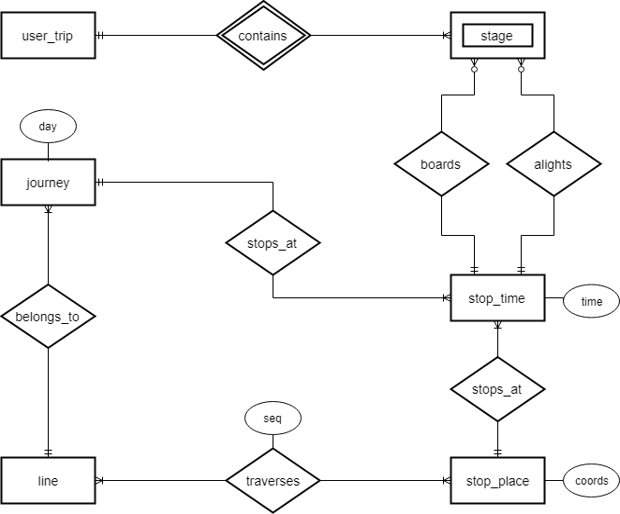
\includegraphics[width=0.75\textwidth]{figures/network_er.png}
        \caption{An ER diagram representing our model of user trips for public transportation networks.}
        \label{fig:er}
        \end{center}
    \end{figure}
    
    These are the main elements from our model:
    \begin{itemize}
        \item A \textbf{stop\_place} is a physical stop with a location, on which several lines may make stops.
        \item A \textbf{line} is an ordered sequence of stop places that can be traveled by a transport vehicle, such as a bus or a train. It only considers one travel direction. For this reason, there is often a different and complementary line for the opposite direction.%, as shown in Figure~\ref{fig:example_network}.
        \item A \textbf{journey} is a singular traversal of a transport vehicle over a line. It can be seen as a vehicle trip, instead of a user trip.
        \item A \textbf{stage} is formed by a boarding from a stop and an alighting to another from the same single line and journey.
        \item An \textbf{user\_trip} is a concatenation of several stages, until the final destination (alighting stop of the last stage) is reached.
    \end{itemize}
	
	This approach allows us to treat the information in a layered fashion: the bottom layer is a static network representation, formed by the line and stop\_place types, the middle layer represents the journeys made by vehicles that make stops at specific times, while the top layer includes the trips made by the users in these vehicle journeys. Finally, it is possible to introduce a \textbf{user} identity, with an anonymized identifier to split trips by users. However, we have not considered such information useful for the kind of analysis that this work focuses on. If needed in the future, this additional entity could be trivially integrated in our representation.
	
	In order to represent and operate our data structures, we will follow this model by defining stops $s_i \in S$, lines $l_i \in L$ and journeys $j_i \in J^l$. It is important to state that journeys are \textbf{not} identified by $j_i$, as the same $j_i$ can belong to several $J^l$ from different lines, so we speak about journey \textbf{codes} (jcodes) instead of journey identifiers. In Figure~\ref{fig:example_trips_ttctr} we can find an example network with two lines and fourteen stops, and journeys that periodically traverse these lines. Note that \mbox{journey-code} 0 appears both in line 0 and in line 1.
	
    \begin{figure}[ht]
        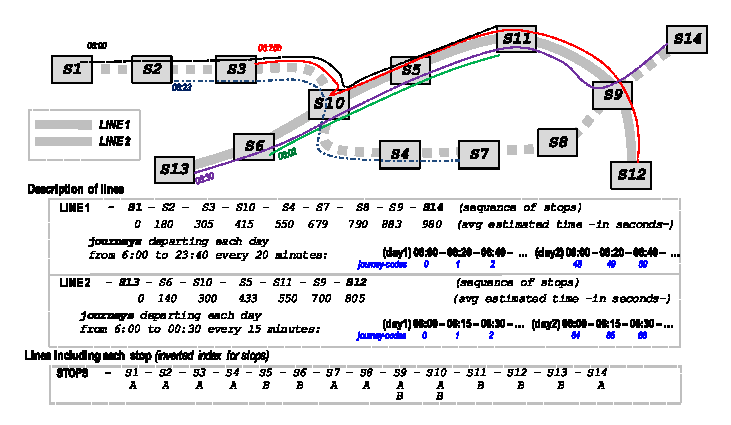
\includegraphics[width=\textwidth]{figures/network.eps}
        \caption{Network representation with the common structures.}
        \label{fig:example_trips_ttctr}
    \end{figure}
    
    A user trip can be represented by the stops from the transportation system that were boarded by a user, so from now on we will consider a trip as a sequence of triplets <$s,l,j$>, where $s$ and $l$ are, respectively, stop and line identifiers, while $j$ are the journey codes corresponding to the journeys that compose the trip. These triplets describe a trip in a consecutive fashion, on the same order as the stops were boarded. Additionally, as we are interested in knowing where the trips end, we also represent the last stop where the user has alighted. Note that both its line and journey will logically match the line and journey of the last boarding stop. Although it is generally hard to obtain information about the last destination stop of a trip, many transportation companies are investing effort in providing it, either by implementing systems to keep track of users as they leave their system or estimating it based on previous trips made by that user \cite{alsger2016validating}.
    
    \medskip
    \begin{example}
    The arrows in Figure~\ref{fig:example_trips_ttctr} are examples of five user trips done along the network.
    For example, there is a user trip (dashed arrow from $S3$) that starts at stop $S3$ at 06:25 on {\em day-1}, 
    %(06:20 + 305 sec.), 
    following the journey $1$ of line $1$ until $S10$, where the user switches to line $2$ at time 06:35 
    %(06:30 + 300 sec.)
    and continues along the journey $2$ of line $2$ (the one started as 06:30 in $S13$) up to stop $S12$. Consequently, this trip includes two stages.
    \qed
    \end{example}
    
    In our first representation, \gls{ttctr}, we encode all valid <$s,l$> pairs into a vocabulary $V$, with every trip defined as a concatenation of the <$s,l$> pairs for the boarded stops, ended by the final destination stop, which will be alighting. We build a \gls{csa} over the concatenation of these trips, and a parallel \gls{wm} with the journey codes of the boarded stops, as previously done for \gls{ctr} in Chapter~\ref{sec:ctr}, but with the temporal component represented by line-dependant journey codes instead of explicit time intervals. For our alternative representation, \gls{xctr}, we only encode the sequence of boarded stops, while the lines go into a parallel \gls{wm}, and the journey codes are in a second \gls{wm} that is aligned to the last level of the first one, allowing us to have more flexibility for some queries, while sacrificing efficiency in others. Finally, \gls{tm} represents a matrix $M^b_l$ for each line $l$ where each cell in the matrix stores the number of boardings (or alightings) performed in the $s$-th stop of the $j$-th journey of line $l$.
	
	\medskip
	In the context of public transportation networks, we are interested in solving two main kinds of queries, which we present with a non-comprehensive list of examples that can be solved with the structures proposed in this work:

    \begin{enumerate}[A)]
        \item Queries about the \textbf{network load}, asking for the gross number of users that boarded or alighted within a stop and a given time/journey. Furthermore, it can be also interesting to obtain the average load of a bus or a train between any two stops from its line. Some of those queries are:
        \begin{itemize}
            \item \boardX$_{LT}$. Number of users that boarded a vehicle at stop X, optionally restricting to a line L and a time range T.
            \item \alightX$_{LT}$. Number of users that alighted a vehicle at stop X, optionally restricting to a line L and a time range T.
            \item \useL$_T$.  Number of users (boarding any vehicle) for the line L, optionally restricting to a time range T.
            \item \boardT.~Number of users boarding (any vehicle) within a time range T.
            \item \alightT.~Number of users alighting (any vehicle) within a time range T.
            \item \loadX$_{LT}$. Average number of passengers traveling from the stop X to its next stop in the line L within the time range T. It can also be seen as the average load of the vehicle.
        \end{itemize}
        
        \item Queries about user \textbf{trips patterns}. With his kind of queries we can obtain the number of times a stop was used to switch lines or the number of trips that started on a stop with another specific stop as the final destination. In this work we consider the following queries of this kind:
        \begin{itemize}
            \item \startX$_{LT}$. Number of user trips starting at a given stop X, optionally restricting to a line L and a time range T.
            \item \endX$_{LT}$. Number of user trips ending at a given stop X, optionally restricting to a line L and a time range T.
            \item \switchX$_{LT}$. Number of trips in which the stop X was used to switch lines, optionally restricting to a destination line L and a time range T.
            \item \texttt{from\_X$_{LT}$\_to\_Y$_{LT}$}. Number of user trips that originate at stop X and end at stop Y, both being optionally restricted to a line and time range. A fundamental difference with the similar definition of \XtoY$_T$ from Section~\ref{sec:ctr:desc} is that we no longer restrict the whole trip to a single time range, but we query for separate time filters for the starting stop $X$ and the ending stop $Y$.
            \item \startL$_T$. Number of user trips starting at any stop from a given line L, optionally restricting to a time range T.
            \item \endL$_T$. Number of user trips ending at any stop from a given line L, optionally restricting to a time range T.
            \item \startT.~Number of user trips starting within a time range T.
            \item \endT.~Number of user trips ending within a time range T.
        \end{itemize}
    \end{enumerate}
	
\section{Structures}
\label{sec:newctr:str}
    To the best of our knowledge, there is no indexing structure that would allow us to efficiently represent trips that could also support all the kinds of queries described in the previous section. For this reason, we propose a new solution that relies on two data structures, \gls{tm}~and~\gls{ttctr}. The former is targeted for queries of type A, solving most aggregation queries in constant time, while the latter can be used for queries of type B. Finally, we introduce a more versatile alternative to \gls{ttctr}~that we call \gls{xctr}.
    
    \subsection{Common Data Structures}
    \label{sec:cs}
    Considering our network formed by stops $s_i \in S$, lines $l_i \in L$, and journeys $j_i \in J^l$, the following structures represent these elements. All our following representations will rely on them.
    
    \begin{itemize}
        \item $lineStop_i(j)$ is the $j$-th stop of line $l_i$.
        \item $stopLine_i(j)$ is the $j$-th line that makes a stop at the stop $s_i$.
        \item $avgTime_i(j)$ is the average time in seconds that it takes for a vehicle of line $l_i$ to reach its $j$-th stop from the start of a journey.
        \item $initialTime_i(k)$ is the starting time of the journey $j_k$ for line $l_i$.
    \end{itemize}
    
    With the exception of $initialTime$, all these structures are considered small enough to be represented using plain fixed-length integer arrays. In the case of $initialTime$, its size naturally grows with the amount of trips that are indexed, thus there is a motivation to reduce its size, which can be easily achieved with any technique that works on posting lists or sequences of strictly increasing numbers, many of which have been discussed and benchmarked in \cite{claude2016universal} and \cite{farina2019reproducibility}. In our work we have used a simplified Vbyte+ANS compression described in \cite{moffat2017ans} using the Zstd library.\footnote{https://github.com/facebook/zstd} In order to facilitate searches and random access, we introduced fixed-length samples on configurable intervals.
    
    Examples of these sequences may be found in Figure~\ref{fig:example_trips_ttctr}, where we indicate the sequence of stops for each line ($lineStop$), the average estimated times ($avgTime$), the initial times of each journey ($initialTime$), and finally the inverted lists of lines per stop ($stopLine$).
    
    \subsection{TTCTR}
    \label{sec:newctr:str:ttctr}
    \acrfull{ttctr}~was introduced in \cite{brisaboa2018new}, as a way of representing trips that are sequences of triplets <$s,l,j$> for every boarded stop $s$, with its line $l$, and journey $j$. Finally, there is also an additional triplet for the last alighted stop, which is considered to be the final destination of the trip. In \gls{ttctr}, the spatial component (the pairs <$s,l$> for the stops and lines of a trip) is represented with a \gls{csa} where each valid pair <$s,l$> is encoded as an integer $id$ in the input sequence $T[1..n]$ that is used to build the \gls{csa}.

    In order to build the \gls{ttctr} structure, all trips must be first sorted. If we consider that a trip is composed by $m$ of the <$s_i,l_i,j_i$>, $1\leq i\leq m$ triplets previously described, where the first triplet corresponds to the first boarded stop and the last triplet corresponds to the last alighted stop (final destination), then the collection of trips is sorted by the key <$s_1,s_m,l_1,j_1$>. That is, trips are initially sorted by the first boarded stop identifier. If these are equal, they are then sorted by their last stop identifier, analogously followed by the line identifier, and journey code of the first stop. 
    %Figure~\ref{fig:example_trips} displays an example of a correct sorting of trips.
    
    \medskip
    \begin{example}
    	By our defined criteria, the correct way of sorting the five trips depicted as arrows in Figure~\ref{fig:example_trips_ttctr} is: 
    	$t_1 = \langle (1,1,0), (10,2,1), (11,2,1)  \rangle$, 
    	$t_2 = \langle (2,1,1), (7,1,1) \rangle$, 
    	$t_3 = \langle (3,1,1), (10,2,2), (12,2,2) \rangle$, 
    	$t_4 = \langle (6,2,0),(11,2,0) \rangle$, and %finally,
    	$t_5 = \langle (13,2,2), (9,1,2), (14,1,2) \rangle$.  
    	
    	Note that, for example, $(13,2,2)$ from $t_5$ indicates that, at stop $13$, the user boarded vehicle from line $2$, that corresponds to the $3$-rd journey (as the first journey-code is zero), which started at 06:30. %We know it is the 2-nd journey because  $t_5$ started at 06:30h, which is the departure time of journey 2.
    	Naturally, the line and journey $ids$ of the last triple of each trip are identical to the ones in the previous triple, as the commuter had to board into that line and journey before alighting from it.
    	\qed \label{ex:trips}
    \end{example}
    
    \medskip
    We also need a bijective function to encode the pairs <$s,l$>. Consider a vocabulary $V$ such that:
    \begin{itemize}
    	\item Entry $V[0]$ is reserved for the terminator symbol $\$$.
    	\item Entries $\langle V[1],V[2], \dots V[|S|]\rangle]$ are associated with stops $s_1,s_2,\dots, s_{|S|}$ and are used to represent the final stops of the trips. That is, when a given stop $s_i$ ends a user trip, it is given $id \leftarrow s_i$.
    	\item The following $|L|\cdot|S|$ entries are associated with the sequence composed of the pairs <$s,l> \in S\times L$, sorted first by the stop id $s$ and later by the line id $l$. That is, entry $V[|S|+1]$ is given to <$s_1,l_1$>; $V[|S|+2]$ to <$s_1,l_2$>; $V[|S|+3]$ to <$s_1,l_3$>; $\dots$; $V[|S|+|L|]$ to <$s_1,l_{|L|}$>;  $V[|S|+|L|+1]$ to <$s_2, l_1$>, $V[|S|+|L|+2]$ to <$s_2, l_2$>, and so on. Therefore, it is easy to see that any <$s_i,l_j$> is going to be associated with the entry $V[|S|+ |L|(i-1) + j]$.
    \end{itemize}
    
    This arrangement would theoretically produce many entries in $V$ that are mapped to pairs <$s,l$> that are unused in $T$, either because the stop is never traversed by that line or (rather unlikely) because we do not have the record of a user trip containing it. These unused entries can be skipped with a compact bitvector $B$ with rank and select capabilities, that marks with a one every used entry from $V$. This will enable us to operate with a much smaller vocabulary $V'$ with only the used entries from $V$, such that $V[i] = V'[\rank_1(B,i)]$. Refer to the vocabulary shown in Figure~\ref{fig:ttctr}(2) for an example where pairs (i.e. <$s,l$>) are encoded to 43 unique identifiers in $V$. After that, $B$ marks which of the entries of $V$ actually appear in the original sequence. Finally. $V'$ will contain only 12 entries, for each bit set to 1 in $B$. Note that neither $V$ nor $V'$ are explicitly represented in practice, as $\rank_1$ and $\select_1$ operations over $B$ are enough to map and unmap, respectively, vocabulary identifiers.

    \begin{figure}[ht]
        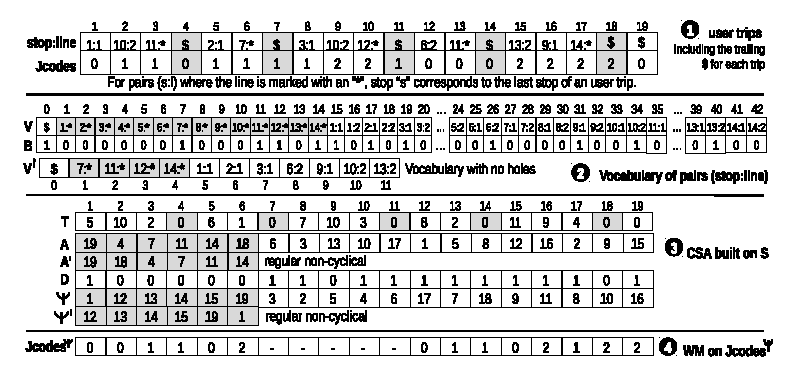
\includegraphics[width=1.00\textwidth]{figures/ttctr2019.eps}
    	\caption{Structures involved in the creation of a \acrshort{ttctr}.}
    	\label{fig:ttctr}
    \end{figure}
    
    After this, the sequence $T[1..n]$ is built, with the identifiers obtained by mapping the pairs <$s,l$> from the user-trips to the vocabulary entries of $V'$. Then a \gls{csa} is built over it, as seen in Figure~\ref{fig:ttctr}(3). Each encoded trip in $T$ is terminated with an additional $\$$ symbol. Even though in the final \gls{csa} we assign all these $\$$ a lexicographical value of 0 $(V[0])$, we assign them different correlative values during the construction of the suffix array (A) to ensure that the entries for $\$$ in $A$ maintain the same order as in the original text. Finally, we make a modification on $\Psi$ to make the entries of each $\$$ point to the start of its own trip instead of the next one (cyclical as in \gls{ctr}, see Section~\ref{sec:ctr:str}). These two modifications are proven necessary for our implemented queries, at the expense of losing some of the properties of a classic \gls{csa} that are not necessary here. For reference, in Figure~\ref{fig:ttctr} we also present $A'$ and $\Psi'$, that show how our modifications compare to the original \gls{csa}.

    The journey codes ($jcodes$) are encoded in $Jcodes^{\Psi}[1..n]$, as shown in Figure~\ref{fig:ttctr}(4), that is aligned to $\Psi$ instead of $T$. $Jcodes[8]= 1$ corresponds to $Jcodes^{\Psi}[14]=1$, since $A[14]=8$; $Jcodes[9]= 2$ corresponds to $Jcodes^{\Psi}[18]=2$, since $A[18]=9$; and so on. Recall that $jcodes$ are relative to their line identifiers, leading us to skip the $jcodes$ that would be aligned to the entries of $\Psi$ belonging to the final stops (represented as ``$s\!:\!*$'' in $V$), as they lack line identifiers, which are in turn needed to identify a journey. Additionally, for the the first positions of $Jcodes^{\Psi}$, aligned with the $\$$ entries, we duplicate the same $jcodes$ as in the beginning of each trip.
	
    Finally, $Jcodes^{\Psi}$ is represented with a \gls{wm}. This is exactly the same strategy as in the case of the temporal component of \gls{ctr}, although in this case we are encoding jcodes instead of time intervals.
    
    \subsection{XCTR}
    \label{sec:newctr:str:xctr}
    For certain queries, \gls{ttctr} can be rather inefficient, as we will discuss later in Section~\ref{sec:newctr:algo}. These use cases motivated us to develop a second version, \gls{xctr}, that instead of encoding the lines into the \gls{csa} vocabulary ($V$), uses a second \gls{wm} with the sequence of line identifiers, thus reducing the complexity of the queries that restrict the final line, and delegates line checks on a new \gls{wm}. This yields improved space-time trade-offs. As in \gls{ttctr}, the input trips need to be sorted by the same criteria, but in \gls{xctr}~we use three complementary structures to represent each component of the sequence, as shown in Figure~\ref{fig:example_xctr}:
    \begin{enumerate}[(i)]
        \item An adapted \gls{csa} over the stop identifiers of all trips, concatenated into a string with additional terminator symbols $\$$ appended at the end of each trip. As in the \gls{csa} from \gls{ttctr}, we make these $\$$ symbols maintain the order of the trips and cyclical in $\Psi$. Because this time we do not encode line and stop identifiers together and \gls{csa} only encodes stops, there is no need for a complex vocabulary anymore.
        \item \texttt{WML}: Aligned to the entries of (i) there is a \gls{wm} for the line identifiers of each stop. Aligned to the $\$$ section we duplicate the starting lines of each trip. As a trivial optimization, we build a separate WM for every stop, allowing us to save space due to the fact that a single stop does not usually belong to many lines, thus the average height of these WM is no larger (and usually smaller) than the height of a single \gls{wm}. In addition, since there are stops that belong to only one line, the corresponding \texttt{WML}s for those stops can be implicitly kept, and therefore they are not actually stored.
        \item \texttt{WMJ}: A \gls{wm} of jcodes aligned to last level of (ii). Note that this makes this structure dependant on (ii), which is coherent with the fact that journey codes themselves are relative to the line identifier. In case (ii) implements the optimization described, the entries of this \gls{wm} must also be rearranged to match the delimited stops.
    \end{enumerate}
    
    \begin{figure}[ht]
    \begin{center}
    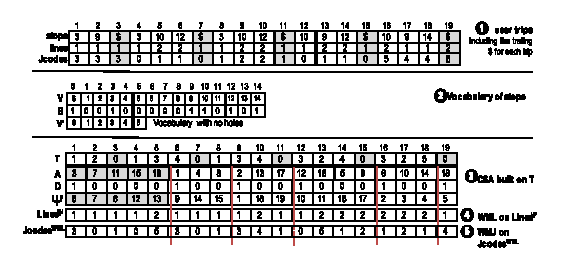
\includegraphics[width=1.00\textwidth]{figures/xctr2019.eps}
    \caption{An example of five trips represented on \acrshort{xctr}~with the optimizations for \texttt{WML} and \texttt{WMJ}, and sections for each stop delimited by dotted lines.}
    \label{fig:example_xctr}
    \end{center}
    \end{figure}
    
    \begin{example}
    Just as in example from Section~\ref{sec:newctr:str:ttctr}, in Figure~\ref{fig:example_xctr} we build \gls{xctr} with five trips over the network shown in Figure~\ref{fig:example_trips_ttctr}. This time, unlike for \gls{ttctr}, our vocabulary $V$ will only contain stop identifiers. These identifiers are used to build the \gls{csa} with our cyclic $\Psi$ variation. Then, the sequence of lines is aligned to the entries of $\Psi$, and \texttt{WML} is built. Note that the only stops used in this example are 0, 3, 9, 10, 12 and 14. Because the stops 3, 12, and 14 belong to only one line each, we do not even need to keep a \gls{wm} for their sections (which are delimited by $D$), as the value will always be the same. This corresponds respectively to the 2-nd, 5-th, and 6-th sections delimited in the figure. Finally, the sequence of Jcodes is aligned to the leaves of \texttt{WML}, and \texttt{WMJ} is built.
    
    For example, <$9,2,1$> from the fourth trip is represented as follows: the stop id $9$ is mapped to $V'[\rank(B,9)-1] = V'[2] = 2$, and it is encoded in $T$ at position $13$. It delimits the $10$-th suffix in the sequence, as $A[10] = 13$, therefore its line identifier $2$ also appears in position $10$ in the sequence $Lines^{\Psi}$. Because in this example we have opted for the optimized version of \texttt{WML}, there is a single \gls{wm} dedicated for the entries of stop $9$, which fall in the section of $A[9..11]$, as delimited by $D$. Therefore, such \texttt{WML} represents the entries $Lines^{\Psi}[9..11] = $<$1,2,1$> and consequently requires only one level that contains the bitmap $010$. This means that in the last (conceptual) level of that \gls{wm} would contain <$1,1,2$> and consequently our entry for line $2$ will appear on the third position. As the sequence $Jcodes^{WML}$ is aligned to this last level of \texttt{WML}, the journey code can be found at $Jcodes^{WML}[11] = 1$.
    \qed \label{ex:xctr}
    \end{example}
    
    \medskip
    In the later Section~\ref{sec:newctr:algo}, we will detail how these structures are used in order to solve the queries proposed in Section~\ref{sec:newctr:desc}, and we will also compare the time complexities with those of \gls{ttctr} for every kind of query.
    
    \subsection{T-Matrices}
    \label{sec:newctr:str:tm}
    While both \gls{ttctr} and \gls{xctr} are effective solutions for the trip pattern queries (type B in Section~\ref{sec:newctr:desc}), they can be too unpractical to efficiently solve network load queries (type A). For this reason, we propose \gls{tm}, a structure based on the \gls{sat} described in Section~\ref{sec:sat}, to which we have designed a compression scheme that will reduce the total size of the structure while maintaining the $O(1)$ time bound for obtaining the sum of an arbitrary rectangle.
    
    We build a \gls{sat} $M^b_l$ for each line $l$, with a column for every stop of that line and a row for every journey, sorted by their starting times. For each cell $M^b_l[j,s]$ we store the number of users that have boarded on the stop $s$ during the journey $j$ from the line $l$. There is also an analogous matrix $M^a_l$ that stores the number of alighting users in $l$. A small example of a single \tm~is displayed in Figure~\ref{fig:tmatrix}, where \textit{Basic} refers to the raw (unaggregated) values, \textit{Sum} are the accumulated values of a \gls{sat}, and \textit{Blocks} is our compressed version.

    \begin{figure}[ht]
    \begin{center}
      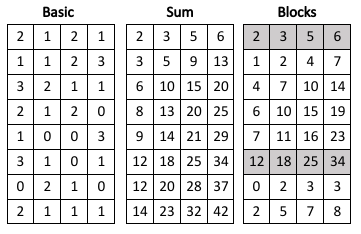
\includegraphics[scale=0.8]{figures/Tmatrices.png}
      \caption{T-Matrices example.}
      \label{fig:tmatrix}
    \end{center}
    \end{figure}
    
    %There are many options for compressing this cumulative matrix in order to get smaller dimensions, in this work we considered two relatively simple options with competitive results. One simple way of dealing with the growth of numbers in our cumulative solution is just apply a kind of sampling with differences; in this way, a basic example could be keep the middle column (\textit{$\mathsf{middle $\leftarrow$  (  \mathopen|c\mathclose|   + 1)/2} $}) explicitly, and representing the values in the other columns \textit{m±k} as the difference with respect to column \textit{m} (Diff in figure \ref{fig:tmatrix}). Being Algorithm to revert this differences as the one shown in Algorithm  \ref{alg:undiff}.
    
    %Taking this simple algorithm one step further we have built a cumulative matrix with several sampling rows, reducing significantly the size of the structure. Hence, this new differential matrix (Blocks in figure \ref{fig:tmatrix}) is divided in square blocks where the first line in each block remains the same as in the cumulative matrix while the rest of the rows in the block are calculated from it. A more technical description would be as follows in the simplified algorithm \ref{alg:unblock}.
    
    In order to compress the size of \gls{tm}, we observe that, because the amount of journeys is usually much larger than the amount of stops in the line, every \gls{tm} is expected to be tall and narrow. Therefore, we can divide the matrix into blocks of $r$ rows, so that only the first row of the block stores the absolute values of a \gls{sat}, while the values in the rest of the rows will be relative to the first one. Given a block matrix $R$ built on the \gls{sat} $S$, any value from $S$ can be then obtained in $O(1)$ time as $S[i,j] = R[\lfloor i/b \rfloor + i\%b,j] + R[i,j]$\footnote{The symbol $\%$ refers to the modulo operation i.e., the remainder of the integer division.} when $i\%b \neq 0$, and $S[i,j] = R[i,j]$ otherwise.

\section{Algorithms}
\label{sec:newctr:algo}
	In these section, we show how the structures from Section~\ref{sec:newctr:str} allow us to solve the queries proposed in Section~\ref{sec:newctr:desc}. Finally, we will provide a complexity analysis that we will later support with experiments in Section~\ref{sec:newctr:exp}.
	
	\subsection{Solving network load queries}
	With \gls{tm}, we can directly solve most of the proposed network load queries with summations over the matrices. For example, \boardX$_{L}$, when we are not restricting to a time interval $T$, is equivalent of summing the corresponding column of the stop $X$ for the matrix $M^b_L$. If we did not want to restrict to a line $L$ either, since there is a $M^b_l$ for every line $l$, we would simply have to add all the sums of those matrices whose lines contain the stop $X$. All this also holds true for \alightX$_{L}$, using the alighting matrix $M^a_L$ instead of the boarding one.
	
	When dealing with queries that do restrict to a time interval $T$, we must find the jcodes of the journeys that will fall within $T$, which can be done with the common structures discussed in Section~\ref{sec:cs}, which store the initial time for each journey and also the average time of arrival to each stop of a line. An example of these structures being used to find a range of jcodes can be found at Algorithm~\ref{alg:jcodes}, where the function \FuncSty{lower\_bound} is an exponential search that returns the index of the first occurrence that is no lesser than the queried value, while \FuncSty{upper\_bound} returns the index of the last no greater occurrence. We also use $lineStop^{-1}_l$(s) to obtain the position of a stop $s$ within the sequence of stops from a line $l$.
    
    \begin{algorithm}[ht]
    \SetKwData{l}{$l$}\SetKwData{lz}{l$_z$}\SetKwData{s}{s}\SetKwData{sz}{s$_z$}\SetKwData{ta}{t$_a$}\SetKwData{tz}{t$_z$}\SetKwData{pattern}{pattern}\SetKwData{left}{left}\SetKwData{right}{right}\SetKwData{csa}{CSA}\SetKwData{wmj}{WMJ}\SetKwData{leftzero}{left$_0$}\SetKwData{rightzero}{right$_0$}\SetKwData{i}{i}\SetKwData{z}{z}\SetKwData{ja}{j$_a$}\SetKwData{jz}{j$_z$}\SetKwData{n}{n}\SetKwData{ap}{a'}\SetKwData{zp}{z'}\SetKwData{offset}{offset}
     \SetKwFunction{GetBounds}{GetBounds}\SetKwFunction{GetJCodes}{GetJCodes}\SetKwFunction{GetCount}{GetCount}\SetKwFunction{GetPsi}{$\Psi$}\SetKwFunction{GetRangeSpecial}{GetRange$^*$}\SetKwFunction{lbound}{lower\_bound}\SetKwFunction{ubound}{upper\_bound}
     \SetKwProg{Fn}{Function}{\string:}{}
     
     \Fn{\GetJCodes{\l,\s,\ta,\tz}}{
     \KwData{line \l, stop \s, times \ta,\tz}
     \KwResult{jcodes for \ta and \tz}
     \BlankLine
     \offset $\leftarrow$ $avgTime_{\l}(lineStop^{-1}_\l$(\s))\;
     \ja $\leftarrow$ \lbound{$initialTime_\l$, \ta-\offset}\;
     \jz $\leftarrow$ \ubound{$initialTime_\l$, \tz-\offset}\;
     \Return{< \ja, \jz>}\;
     }
     
     \caption{Obtaining the codes of the journeys from the line $l$ that should arrive to the stop $s$ within the time range given by t$_a$ and t$_z$.}
     \label{alg:jcodes}
    \end{algorithm}
    
    The range of jcodes obtained $[j_a..j_z]$ will correspond to a range of rows in the \tm~of the queried line, thus allowing us to solve \boardX$_{LT}$ (or \alightX$_{LT}$) as a sum of the rectangle $M^b_L[j_a..j_z, s]$ (or $M^a_L[j_a..j_z, s]$), where $s$ is the corresponding column for the stop $X$. Similarly, we can solve \useL$_T$ with a summation on the last column of $L$, restricted to the range of jcodes of $T$.
    
    Finally, we can solve \loadX$_{LT}$ by combining both the boarding and the alighting matrices, with the observation that at any stop $X$, the number of passengers in the vehicle has to equal the number of passengers that had boarded at or before $X$ minus the number of passengers that had alighted. Therefore, for any line $L$, a range of stop indices $[s_a..s_z]$ that occur in $L$ until $X$, and a range of jcodes $[j_a..j_z]$ obtained for $T$, it follows that 
    \[\loadX_{LT} = 
    \displaystyle\sum_{s \in [s_a..s_z]}
    \displaystyle\sum_{j \in [j_a..j_z]}
    M^b_L[j,s] - M^a_L[j,s]\]
    , which can be computed in $O(1)$ because we refer to a contiguous range in $M^b_L$ and $M^a_L$.
	
	\subsection{Solving trip pattern queries}
	\label{sec:newctr:algo:xy}
	As with \gls{ctr}, we also obtain a clear separation between the spatial representation of the trips (\gls{csa}) and the temporal representation (\gls{wm} of $Jcodes^{\Psi}$) in \gls{ttctr}. The spatial component can be used to address queries such as ``number of passengers that started their trip from a stop $X\in S$ and a line $l\in L$'' (\texttt{\startX$_{L}$} from Section~\ref{sec:newctr:desc}) with a binary search of the pattern $\$X_l$, as the pair <$X,l$> will be mapped to a single symbol $X_l$ in $V$. The temporal component can be used to filter down these results to a time window (\texttt{\startX$_{LT}$}) with a $\cnt_{j_a,j_z}(Jcodes^{\Psi},i,j)$ operation over the \gls{wm}, where $j_a$ and $j_z$ are $jcodes$ obtained from Algorithm~\ref{alg:jcodes} and $i$ and $j$ delimit the range of the results obtained in $\Psi$. Because the $\$$ symbols were made cyclical in $\Psi$, it is also possible to answer \texttt{from\_X\_to\_Y} queries by searching for a pattern $Y\$X_l$ instead.
	
	With \gls{xctr} we can overcome the main weakness of \gls{ttctr}, i.e. that it requires several binary search operations over the \gls{csa} in the following cases:
    \begin{itemize}
        \item We are interested in the number of passengers that started their trip at a stop $X$ and a time window $t_a..t_z$, but from \textbf{any line} (\texttt{\startX$_{T}$}). As $jcodes$ are relative to lines, we must make a separate query for each possible pair <$X, l_i> \forall l_i \in L$.
        \item We need to restrict the line of a final stop, in queries such as \texttt{\endX$_{L}$} or \texttt{from\_X\_to\_Y$_{L}$} (and similar variations). Because the final stops belong to separate entries of the vocabulary that do not encode line identifiers, to restrict a stop $Y\in S$ to a line $l\in L$ we need to search for every possible expanded pattern $W_l,Y...$, for every stop $W$ from the line $l$ that could have been boarded before alighting at $Y$. While it looks tempting to address this issue by modifying the design of \gls{ttctr}~so that final stops also encode line identifiers, this would in turn make queries that do not restrict the line of the final stop inefficient, and we would need to perform a new query for every combination of $(Y, l_i)~\forall l_i \in L$, as in the previous case.
    \end{itemize}
	
	We address these limitations in \gls{xctr}, at the expense of an additional structure, which involves more (conceptual) complexity in our operations. We will now proceed to detail how a single trip $t_i$ may be extracted from this compact representation
	%is also a complete representation of the collection of trips, we are able to extract any trip using the structures described. 
	in Algorithm~\ref{alg:extract}, where 
	%\FuncSty{Rank} and \FuncSty{Select} operate over the bitvector $D$ from our \gls{csa}, 
	\FuncSty{WML}{(s$_a$)} is the WM corresponding to the stop \DataSty{s$_a$} in the optimized version of \texttt{WML}\footnote{Recall that the optimized \texttt{WML} keeps a separate \gls{wm} for every stop, instead of a single one for all the line identifiers. Without this optimization, the pseudocode would still be valid by assigning $z\leftarrow 0$ at line 6.} and \FuncSty{TrackDown} returns the leaf index of a WM given a root index. In a practical implementation, it is not needed to access \texttt{WML} and \texttt{WMJ} for the line identifier and jcode of the last stop of the trip, as they will always match the previous ones.
	
	\begin{algorithm}[h!]
    \SetKwData{la}{$l_a$}\SetKwData{lz}{$l_z$}\SetKwData{sa}{s$_a$}\SetKwData{sz}{s$_z$}\SetKwData{ta}{t$_a$}\SetKwData{tz}{t$_z$}\SetKwData{pattern}{pattern}\SetKwData{left}{left}\SetKwData{right}{right}\SetKwData{csa}{CSA}\SetKwData{leftzero}{left$_0$}\SetKwData{rightzero}{right$_0$}\SetKwData{a}{a}\SetKwData{z}{z}\SetKwData{ja}{j$_a$}\SetKwData{jz}{j$_z$}\SetKwData{n}{n}\SetKwData{ap}{a'}\SetKwData{zp}{z'}\SetKwData{offset}{offset}\SetKwData{i}{i}\SetKwData{trip}{trip}
     \SetKwFunction{GetRange}{GetRange}\SetKwFunction{GetJCodes}{GetJCodes}\SetKwFunction{GetCount}{GetCount}\SetKwFunction{GetPsi}{$\Psi$}\SetKwFunction{GetRangeSpecial}{GetRange$^*$}\SetKwFunction{wml}{WML}\SetKwFunction{TrackUp}{TrackUp}\SetKwFunction{fxy}{FromXtoY\_full}\SetKwFunction{extract}{Extract\_trip}\SetKwFunction{TrackDown}{TrackDown}\SetKwFunction{wmj}{WMJ}
     \SetKwProg{Fn}{Function}{\string:}{}
     
     \Fn{\extract{\i}}{
     \KwData{trip number \i}
     \KwResult{Sequence of tuples <$s,l,j$> that compose the trip}
     \BlankLine
     \trip $\leftarrow~[]$\;
     \a  $\leftarrow~\GetPsi[\i]$\;
     \sa $\leftarrow~\rank_1(D,\a)$\;
     \BlankLine
     \While{\sa $\neq$ 0}{
        \z $\leftarrow~\select_1(D,\sa)$\;
        \la $\leftarrow~\wml{\sa}[\a-\z]$\;
        \ja $\leftarrow~\wmj[\TrackDown{\wml{\sa}, \a-\z}+\z]$\;
        append $<\sa,\la,\ja>$ to \trip\;
        \a  $\leftarrow~\GetPsi[\i]$\;
        \sa $\leftarrow~\rank_1(D,\a)~-~1$\;
     }
     \BlankLine
     \Return{\trip}\;
     }
     
     \caption{Extracting the trip \DataSty{i} from \acrshort{xctr}, using its components $\Psi$, $D$, \FuncSty{WML} and \FuncSty{WMJ} from Figure~\ref{fig:example_xctr}.}
     \label{alg:extract}
    \end{algorithm}
    
    Note that Algorithm~\ref{alg:extract} starts with the first stop of the trip, for which it recovers the corresponding line $l_a$ and journey $j_a$. Then, it continues with the next stop of the trip in line 10, until the ending $\$$ (a 0) is reached.
    
    A more complex example of these structures working together is the query ``number of trips that started from a stop \DataSty{s$_a$} and ended at a stop \DataSty{s$_z$}'', which can be further restricted to specific starting and ending lines and a time window (\texttt{from\_X$_{LT}$\_to\_Y$_{LT}$}). The pseudocode for the full version of such query can be found in Algorithm~\ref{alg:xy}. This algorithm relies heavily on the $\cnt_{j_a,j_z}(Jcodes^{\Psi},i,j)$ operation, as well as its variant $\cnt^{LR}$, both defined in Section~\ref{sec:wt}.
    
    \begin{algorithm}[h!]
    \SetKwData{la}{$l_a$}\SetKwData{lz}{$l_z$}\SetKwData{sa}{s$_a$}\SetKwData{sz}{s$_z$}\SetKwData{ta}{t$_a$}\SetKwData{tz}{t$_z$}\SetKwData{pattern}{pattern}\SetKwData{left}{left}\SetKwData{right}{right}\SetKwData{csa}{CSA}\SetKwData{leftzero}{left$_0$}\SetKwData{rightzero}{right$_0$}\SetKwData{a}{a}\SetKwData{z}{z}\SetKwData{ja}{j$_a$}\SetKwData{jz}{j$_z$}\SetKwData{n}{n}\SetKwData{ap}{a'}\SetKwData{zp}{z'}\SetKwData{offset}{offset}
     \SetKwFunction{GetJCodes}{GetJCodes}\SetKwFunction{GetCount}{GetCount}\SetKwFunction{GetPsi}{$\Psi$}\SetKwFunction{GetRangeSpecial}{GetRange$^*$}\SetKwFunction{wml}{WML}\SetKwFunction{TrackUp}{TrackUp}\SetKwFunction{fxy}{FromXtoY\_full}\SetKwFunction{wmj}{WMJ}
     \SetKwProg{Fn}{Function}{\string:}{}
     
     \Fn{\fxy{\la,\lz,\sa,\sz,\ta,\tz,\n}}{
     \KwData{lines \la,\lz, stops \sa,\sz, times \ta,\tz and length of the sequence \n}
     \KwResult{Number of occurences}
     \BlankLine
     %\pattern $\leftarrow [\sz,0,\sa]$\;
     $[\left,\right]~\leftarrow~\bsearch(\Psi, \sz\$\sa)$\;
     \leftzero $\leftarrow~\GetPsi[\left]$\;
     \rightzero $\leftarrow~\GetPsi[\right]$\;
     \tcp{\right-\left = \rightzero-\leftzero}
     $[\a,\z]~\leftarrow~\cnt^{LR}_{\la,\la}(\wml{\$},\leftzero,\rightzero)$\;
     \tcp{$\leftzero \leq \a \leq \z \leq \rightzero$}
     $[\ja,\jz]~\leftarrow$ \GetJCodes{\la,\sa,\ta,\tz}\;
     $[\a,\z]~\leftarrow~\cnt^{LR}_{\ja,\jz}(\wmj,\TrackDown{\a},\TrackDown{\z})$\;
     \ap $\leftarrow$ \TrackUp{\wml{$\$$},\a}\;
     \zp $\leftarrow$ \TrackUp{\wml{$\$$},\z}\;
     \tcp{\z-\a = \zp-\ap}
     \offset $\leftarrow~\select_1(D,\sz)$\;
     $[\a,\z]~\leftarrow~\cnt^{LR}_{\lz,\lz}(\wml{\sz},\left-\offset+\ap-\leftzero,
     \left-\offset+\zp-\leftzero)$\;
     $[\ja,\jz]~\leftarrow~\GetJCodes{\lz,\sz,\ta,\tz}$\;
     \Return{$\cnt_{\ja,\jz}(\wmj,\offset~+~\a,\offset~+~\z)$}\;
     }
     
     \caption{Querying for \texttt{from\_X$_{LT}$\_to\_Y$_{LT}$} with all restrictions on \acrshort{xctr}.}
     \label{alg:xy}
    \end{algorithm}
    
    \medskip
    We will now proceed to explain the process in Algorithm~\ref{alg:xy} line by line:
    \begin{itemize}
        \item In \textbf{line 2}, we query our \gls{csa} for the pattern consisting of the destination stop \DataSty{s$_z$}, followed by a $\$$ and finally the origin stop \DataSty{s$_a$}. This results in a range of entries within the section of \DataSty{s$_z$} that belong to our queried trips, because the trips were made circular in $\Psi$, so each $\$$ points to the beginning of its own trip. If we were not interested in restricting lines nor time, the function would end here, returning \DataSty{right}-\DataSty{left}.
        
        \item In \textbf{lines 3-5} we obtain the corresponding range in the section of $\$$ by accessing \FuncSty{$\Psi$}. Note that because of how the sorting of the $\$$ symbols was altered during the construction of the suffix array, these two ranges are equal in size, as the comment in line 5 points out.
        
        \item In \textbf{line 6} we query \texttt{WML} in the $\$$ section, within the range previously obtained, for the queried starting line \DataSty{$l_a$}, obtaining the range of its occurrences $[$\DataSty{a}$..$\DataSty{z}$] \subseteq [$\DataSty{left}$_0..$\DataSty{right}$_0]$, since the $\$$ were sorted by their starting stop first, ending stop second and their starting line third. Note that if the \gls{xctr}~were constructed without the optimization that separates \texttt{WML} in sections, this line would be exactly the same, except for the query being on a \DataSty{WML} that would encode the whole sequence of lines instead of just the \DataSty{WML}{($\$$)} for $\$$.
        
        \item In \textbf{line 8} we obtain the range of jcodes for the journeys from the line \DataSty{$l_a$} that would pass through the stop \DataSty{s$_a$} within the time window delimited by \DataSty{t$_a$} and \DataSty{t$_z$}, using the function \FuncSty{GetJCodes} from Algorithm~\ref{alg:jcodes}.
        
        \item In \textbf{line 9} we operate over a range of \texttt{WMJ} that encodes a non-decreasing sequence of jcodes, given that within the same origin stop, final stop, and starting line, the $\$$ symbols were sorted by the starting journey code of their trips. This allows us to keep using $\cnt^{LR}$, as we are still operating within the $\$$ section. We also need to use \FuncSty{TrackDown} on \DataSty{a} and \DataSty{z} since \FuncSty{WMJ} is aligned to the last level of \FuncSty{WML}.
        
        \item In \textbf{lines 10-12} we use the \FuncSty{TrackUp} operation, which is the inverse of \FuncSty{TrackDown}: it returns the position in the first level given a position in the last level of a WM. In this case, as the \FuncSty{a} and \FuncSty{z} we obtained in the previous step are also positions in the last level of the \FuncSty{WML}, we use \FuncSty{TrackUp} to translate that range of indexes to the root of \texttt{WML} and therefore to the entries of the \gls{csa} as well. Note that the resuling range is inside the $\$$ section for trips with the same origin stop, final stop, and starting line that includes all the trips for jcodes that span from \DataSty{j$_a$} to \DataSty{j$_z$}. The properties of our adapted \gls{csa} also ensure that this range maintains the same size after translation and it can also be directly translated to a range in $[$\DataSty{left}$..$\DataSty{right}$]$.
        
        \item In \textbf{line 13} we obtain the starting position of the section for the stop \DataSty{s$_z$} in the \gls{csa} with a $\select_1$ operation over the bitvector $D$. This is necessary for operating on \texttt{WML} and \texttt{WMJ} to restrict the line and journeys for the final stop.
        
        \item In \textbf{line 14} the range $[$\DataSty{a'}$..$\DataSty{z'}$] \subseteq [$\DataSty{left$_0$}$..$\DataSty{right$_0$}$]$ is trivially translated to the section for
        \DataSty{s$_z$} within $[$\DataSty{left}$..$\DataSty{right}$]$, where we query \texttt{WML} to obtain the subrange $[$\DataSty{a}$..$\DataSty{b}$] \subseteq [$\DataSty{left}$..$\DataSty{right}$]$ for the line \DataSty{l$_z$}. Remember that \FuncSty{WML}(s$_z$) represents only the lines for \DataSty{s$_z$}, therefore both the translated positions and the resulting subrange positions are relative and must be adjusted by \DataSty{offset}. This would have not been necessary if the optimization was not implemented, and absolute positions would have been used (\DataSty{offset}$\leftarrow 0$).
        
        \item In \textbf{line 15} we obtain the jcode range analogously to line 8, but this time for \DataSty{$l_z$} and \DataSty{s$_z$}.
        
        \item In \textbf{line 16} we return the number of entries of \texttt{WMJ} between \DataSty{j$_a$} and \DataSty{j$_z$} within our final subrange. Unlike $\cnt^{LR}$, $\cnt$ does not report any range boundaries, but simply returns the number of occurrences.
    \end{itemize}
    
    It is trivial to reuse Algorithm~\ref{alg:xy} to answer queries with less constrains. For example, if we were only interested in restricting the starting line, we could return \DataSty{z}-\DataSty{a} after line 6. If we only wanted to restrict the ending line and time, we could do it by skipping the lines 3-12, and using directly $\cnt^{LR}_{l_z,l_z}(\FuncSty{WML}($\DataSty{s}$_z),$\DataSty{left-offset,right-offset}$)$ in line 14. 
    
    The complexity would increase if we restricted by a time window but not by lines, as we would need to iterate through all possible lines for \DataSty{s$_a$} and \DataSty{s$_z$} to obtain the jcodes for each line and perform these operations on \texttt{WML} and \texttt{WMJ}. Fortunately, the number of lines a single stop can belong to tends to be rather small in practice, thus with a careful implementation that avoids repeating computation, the performance of such query scales well, as it will be shown later in Section~\ref{sec:newctr:exp}. Finally, to obtain only the trips that started on a given stop we would simply need to set \DataSty{pattern} to $\$s_a$ in line 2, or alternatively to $s_z\$$ for the final stop, and skipping the operations on the sections of \DataSty{s$_z$} or $\$$, respectively.
    
    \medskip
    Additionally, \gls{xctr}~can also be used to efficiently obtain other interesting information about trips, such as the top k most boarded stops, 
    %as shown in \cite{brisaboa2018compact} \ojo{NO}, 
    with the possibility of differentiating stops that are only used to switch lines in \gls{xctr}. However, to the best of our knowledge, there exists no efficient way of using this representation to obtain other kinds of information efficiently (e.g. the number of passengers in a journey between two stops).
	
	\subsection{Analyzing our representations}
	\label{sec:newctr:algo:analysis}
	To illustrate the application of each representation, as well as highlight the motivation for the development of \gls{xctr}, in this section we discuss in detail the worst case time complexities of each query described in Section~\ref{sec:newctr:desc}, being $l$ the number of lines we restrict to, $|L|$ the total number of lines represented, $|S|$ the number of stops in the queried line and $|J^l|$ is the maximum number of jcodes per line.
    
    \begin{threeparttable}
    \centering
    \begin{tabular}{|c|l|l|l|l|}
    \hline
    & Query &  \gls{tm} & \gls{ttctr} & \gls{xctr}\\
    \hline
    \multirow{6}{*}{\rotatebox[origin=c]{90}{\centering Type A}}
    & \texttt{\boardX$_{LT}$} & $O(l)$ & $O(l\cdot \log(|J^l|))$ & $O(\log(n |L|\cdot |J^l|))$\tnote{$\otimes$} \\
    & \texttt{\alightX$_{LT}$} & $O(l)$ & Hard\tnote{$\ddagger$$\diamondsuit$} & Hard\tnote{$\ddagger$$\diamondsuit$} \\
    & \texttt{\useL$_T$} & O(1) & $O(|S|\log(|J^l|))$ & $O(|S|\log(n |L|\cdot |J^l|))$\tnote{$\otimes$} \\
    %\texttt{alight\_L$_T$} & O(1) & $O(|S|\log(|J^l|))$\tnote{$\otimes$$\ddagger$} & $O(|S|\cdot $O(\log(n |L|\cdot |J^l|))$)$\tnote{$\otimes$$\ddagger$} \\
    & \texttt{\boardT} & $O(|L|))$ & Hard\tnote{$\diamondsuit$} & Hard\tnote{$\diamondsuit$} \\
    & \texttt{\alightT} & $O(|L|)$ & Hard\tnote{$\ddagger$$\diamondsuit$} & Hard\tnote{$\ddagger$$\diamondsuit$} \\
    & \texttt{load\_X$_{LT}$} & $O(l)$ & Hard\tnote{$\ddagger$$\diamondsuit$} & Hard\tnote{$\ddagger$$\diamondsuit$} \\
    \hline
    \multirow{8}{*}{\rotatebox[origin=c]{90}{\centering Type B}}
    & \texttt{\startX$_{LT}$} & - & $O(\log(n|J^l|))$\tnote{$\otimes$} & $O(\log(n |L|\cdot |J^l|))$\tnote{$\otimes$} \\
    & \texttt{\endX$_{LT}$} & - & $O(|S|\log(n|J^l|))$\tnote{$\otimes$} & $O(\log(n |L|\cdot |J^l|))$\tnote{$\otimes$} \\
    & \texttt{\switchX$_{LT}$} & - & $O(\log(n|J^l|))$\tnote{$\otimes$} & $O(\log(n |L|\cdot |J^l|))$\tnote{$\otimes$} \\
    & \texttt{from\_X$_{LT}$\_to\_Y$_{LT}$} & - & $O(|S|\log(n|J^l|))$\tnote{$\otimes$} & $O(\log(n |L|\cdot |J^l|))$\tnote{$\otimes$} \\
    & \texttt{\startL$_T$} & - & $O(|S|\log(n|J^l|))$\tnote{$\otimes$}~~ & $O(\log(|L|\cdot |J^l|))$ \\
    & \texttt{\endL$_T$} & - & Hard\tnote{$\diamondsuit$} & $O(|S|\log(n |L|\cdot |J^l|))$\tnote{$\otimes$} \\
    & \texttt{\startT} & - & Hard\tnote{$\diamondsuit$} & $O(|L|\log(|L|\cdot |J^l|))$~~ \\
    & \texttt{\endT} & - & Hard\tnote{$\diamondsuit$} & Hard\tnote{$\diamondsuit$} \\
    \hline
    \end{tabular}
    
    \begin{tablenotes}
    %\item[a] $l$ is the number of lines we restrict to.
    \item[$\otimes$] The complexity will increase when the line is not restricted. See discussion.
    \item[$\ddagger$] May include false positives.
    \item[$\diamondsuit$] Not practical to solve with the indexing capabilities of this representation.
    %\item[e] $|S|$ is the number of stops in the line L.
    %\item[f] $|L|$ is the total number of lines represented.
    %\item[g] $|J^l|$ is the average number of jcodes per line.
    \end{tablenotes}
    
    \caption{Worst case time complexities for the representations described in Section~\ref{sec:newctr:str}, assuming the queries have all the restrictions.}
    \label{tab:queries}
    \end{threeparttable}
    
    \medskip
    Before explaining the details of how each of these operations would be implemented in our representations, it is worth noting that the complexity of the \gls{xctr} and \gls{ttctr} queries marked by $\otimes$ will depend on the constraints that are applied, as explained in the previous Section~\ref{sec:newctr:algo:xy}. Generally, the time complexity of \gls{xctr} with all the restrictions is bounded by one $\bsearch$ operation on the \gls{csa} to restrict by a stop id, one $\cnt^{LR}$ on \FuncSty{WML} to restrict by a line id and, finally, a $\cnt$ on \FuncSty{WMJ} to restrict by jcodes, with a total complexity of $O(\log(n |L|\cdot |J^l|))$, being $n$ the size of the represented sequences.\footnote{While theoretically locating a pattern of length $m$ in a Suffix Array takes $O(m \log n)$ time, in our case $m$ is bounded to 2 or 3 (in case of \texttt{from\_X\_to\_Y}). Furthermore, with a backward search implementation, only $m-1$ binary searches are needed.}
    However, when only the time is restricted, every line that the queried stop belongs to must be considered, thus increasing the worst-case complexity to $O(\log(n) + |L|\log(|L|\cdot |J^l|))$. Similarly, the complexity of \gls{ttctr} is normally a search in the \gls{csa} and a $\cnt$ on the \gls{wm} (if time is restricted), which would amount to $O(\log(n|J^l|))$, although when only the time (and not the line) is restricted, we must perform a new query for every possible line, and the complexity increases to $O(|L|\log(n|J^l|))$, which is generally higher than $O(\log(n) + |L|\log(|L|\cdot |J^l|))$, the one from \gls{xctr}.
    
    \begin{itemize}
        \item \texttt{\boardX$_{LT}$}. This can be solved easily in the \gls{tm}, as there are aggregated matrices for boarding stops, even though it is necessary to access a separate matrix for every line queried, hence $O(l)$. For \gls{ttctr}, the number of occurrences for the stop $X$ is counted by delimiting its range in $D$ (with a $O(1)$ $\select_1$ operation) and filtering down the \gls{wm} if needed. For \gls{xctr}, the filtering is done through \FuncSty{WML} and \FuncSty{WMJ}, and after that we must subtract the occurrences of final stops, obtained by one \texttt{\endX$_{LT}$} with the same restrictions.
        \item \texttt{\alightX$_{LT}$}. Both in \gls{ttctr}~and \gls{xctr}, the only alighting stops that are explicitly represented are the final stops. To obtain an approximated count of the rest of them, we would need to extract and examine all the occurrences for \texttt{board\_W$_{LT}$} for every stop W that could have been boarded before X, as the worst-case time complexity of solving with their index operations is prohibitive. On the other hand, it can be solved much faster in \gls{tm}~by accessing the alighting matrices.
        \item \texttt{\useL$_T$}. This operation is straightforward to solve in \gls{tm}, as it only needs to access one matrix. For \gls{ttctr}~we must filter through the \gls{wm} for every stop from L. While in \gls{xctr}~the total number of occurrences of line L can be calculated in one $O(\log|L|)$ operation (with additional filtering through \FuncSty{WMJ} if needed), we need to subtract the occurrences of \startL$_T$ and \endL$_T$, the latter having a higher complexity of $O(|S|\log(n |L|\cdot |J^l|))$.
        %\item \texttt{alight\_L$_T$} Can be approximated both in \gls{ttctr}~and \gls{xctr}~with board\_L$_T$, given that every user that boards on a line is expected to alight from it within a reasonable time.
        \item \texttt{\boardT~and~\alightT}. Although \gls{tm}, \gls{ttctr},~and \gls{xctr}~could solve it by applying \useL$_T$ $|L|$ times, this would imply a prohibitive cost for both \gls{ttctr}~and \gls{xctr}, where extracting all the trips would be preferred in practice.
        \item \texttt{load\_X$_{LT}$}. It is possible to solve this kind of query using both alighting and boarding matrices in \gls{tm}. Knowing how many travelers got on and off the vehicle previously to one particular point makes trivial to determine how many of them are in the vehicle between two stops. This method can be easily adapted to measure the average number through an interval of time.
    \end{itemize}
    
    \medskip
    The following Type B operations are not supported by \gls{tm}:
    
    \begin{itemize}
        \item \texttt{\startX$_{LT}$}. We need to the range for the pattern $\$X$ in the \gls{csa} and to filter down the \gls{wm}s, if needed.
        \item \texttt{\endX$_{LT}$}. In \gls{xctr}~it is solved similarly to \texttt{\startX$_{LT}$}, by delimiting the range for the pattern $X\$$ in the \gls{csa} and to filter down \gls{wm}s, if needed. It can be much more complex for \gls{ttctr}, where the only way to restrict a line is to make a new query for every stop that could have been boarded before X in that line, which is a problem detailed at the begining of Section~\ref{sec:ctr}.
        \item \texttt{\switchX$_{LT}$}. It is calculated as \boardX$_{LT}$ - \startX$_{LT}$.
        \item \texttt{from\_X$_{LT}$\_to\_Y$_{LT}$}. It was explained in detail in Algorithm~\ref{alg:xy}. In \gls{ttctr}~the $|S|$ factor only takes effect if the line (or time) for Y must be restricted, as for \texttt{\endX$_{LT}$}.
        \item \texttt{\startL$_T$}. It is trivially solved in \gls{xctr}, by filtering down \FuncSty{WML} and \FuncSty{WMJ}, if needed, over the $\$$ section of the \gls{csa}. On the other hand, for \gls{ttctr}~the \gls{csa} needs to be queried with the $\$X$ pattern for every stop X from line $l$.
        \item \texttt{\endL$_T$}. It can be solved in \gls{xctr}, by performing a \endX$_{LT}$ for every stop X from the line $l$. If we used the same strategy for \gls{ttctr}, we would end up with a complexity of $O(|S|^2\log(n|J^l|))$, which we consider prohibitive.
        \item \texttt{\startT}. It is solved in the \gls{xctr}~by applying \texttt{\startX$_{LT}$} $|L|$ times.
        \item \texttt{\endT}. None of our representations can solve this query efficiently, although it could be approximated by \texttt{\startT}.
    \end{itemize}
	
\section{Experiments}
\label{sec:newctr:exp}
	In this section we discuss the practical performance of our structures. To evaluate them, we have run randomly generated queries against \gls{tm}, \gls{ttctr},~and \gls{xctr}~built over a dataset of synthetic user trips generated from a real transportation network (Section~\ref{sec:newctr:exp:data}), with several configurations to study the trade-off between compression (Section~\ref{sec:newctr:exp:space}) and query efficiency (Section~\ref{sec:newctr:exp:time}), and testing different configurations for each individual structure.

    \subsection{Experimental dataset}
    \label{sec:newctr:exp:data}
    Using real GTFS\footnote{\url{https://developers.google.com/transit/gtfs/}} descriptions of bus routes and schedules, we generated a synthetic dataset of user trips that aims to realistically imitate real user behaviour during a month. In this work, we have combined the GTFS obtained for the networks of urban\footnote{Provided by EMT \url{http://www.emtmadrid.es}} and interurban\footnote{Provided by CRTM \url{http://www.crtm.es}} buses for the city of Madrid. The network model was extracted and user trips were generated with the following general steps:
    
    \begin{enumerate}
        \item We parsed stop, route, and trip identifiers. This produced two lines per route in almost all cases, one for each direction. With the gathered data, we were able to build the common structures $lineStop$ and $stopLine$ discussed in Section~\ref{sec:cs}.
        \item We connected stops that are on a short walking distance (100 meters) from each other, or appear sequentially on the same line.
        \item We parsed the schedules for bus trips.
        \item We generated a month of journeys from the schedules, differentiating days of week. From this step, we computed $avgTime$ and $initialTime$ common structures.
        \item User trips were generated. A trip starts from a random stop, day, and journey and simulates boarding that journey and traversing it. After each traversed stop, the user may end the trip with a probability that starts at zero and increases by 1\% for every stop visited. Additionally, there is a fixed probability of attempting to switch lines at the current stop, if there is a journey available at that stop within the allowed waiting time (30 minutes) and from a different line.\footnote{The reverse of the current line is also disallowed.} Switching lines is also attempted when the end of the current line is reached.
        \item We persisted these generated trips as sequences of stages \\ < <$line,journey,boarding\_stop$>, <$line,journey,alighting\_stop$> >,\\ where a boarding and alighting stop naturally share the same line and journey within the same stage. This results in the same number of stages as lines have been used. With the parameters used, about 56\% of our trips have one stage, 33\% have two, 9\% have three, and 2\% have four.
    \end{enumerate}
    
    With this approach we have generated a dataset of ten million trips, over a real network consisting of 11021 stops, 1048 lines for a simulated month,\footnote{A period of 31 days, starting on a Monday.} with an average of 1622 journeys per line and a maximum of 9980 per line. We consider that this synthetic dataset is of enough accuracy and size to obtain significant results when studying the compression capabilities and performance of our representations.
    
    \subsection{Space requirements}
    \label{sec:newctr:exp:space}
    We have measured the \mbox{in-memory} sizes of all the individual components of our representation built over the experimental dataset. We also present the sizes of our common structures, followed by \gls{tm}. After that, we compare the compression achieved with \gls{ttctr}~and \gls{xctr}.
    
    For the \gls{csa} structures from \gls{ttctr}~and \gls{xctr}, we use an adapted $iCSA$ from \cite{FBNCPR12}, and tuned it with the $t_\Psi$ (sampling interval) factors of 32, 128, and 512. For the \gls{wm} present in \gls{ttctr}, as well as in the two \gls{wm} from \gls{xctr}, we analyze the space required by four different configurations: when we tune the \gls{wm}s to use the \texttt{RRR} bitvector and tuning it to use 
    %described in \cite{Raman:2002:SID:545381.545411}, using block sizes of 32, 64 and 128, and compare it against
    a plain bitvector with a rank structure, which we call \texttt{RG32}.
    
    The space occupied by the common structures is reflected in Table~\ref{tab:commons}. These were represented using plain fixed bit length integers with the exception of $initialTime$, where we used the compression approach discussed in Section~\ref{sec:cs} with a sampling interval of 512. This has allowed us to represent all required network information in a negligible space of less than 1 MiB.
    
    \begin{table}[ht]
        \centering
        \begin{tabular}{|c|c|c|c|c|c|}
        \hline
            Structure & $lineStop$ & $stopLine$ & $avgTime$ & $initialTime$ & Total \\
            \hline
            Size (KiB) & 119 & 141 & 64 & 440 & 764 \\
        \hline
        \end{tabular}
        
        \caption{Sizes of the common structures.}
        \label{tab:commons}
    \end{table}
    
    To measure the amount of space occupied by the two different variants of \gls{tm}~that were presented in Section~\ref{sec:newctr:str:tm}, we have summed the total space required by each line matrix. These results, which can be found in Table~\ref{tab:acuum}, helped us to prove that \texttt{Blocks} is an effective strategy to reduce the size of the accumulated values. %While \texttt{Diff} is also able to reduce the total space, it's fundamentally constrained by the shape of our matrices, making it less desirable in this context.
    
    \begin{table}[ht]
        \centering
        \begin{tabular}{|c|c|c|c|}
        \hline
            Variant & \texttt{Sum} & \texttt{Blocks} \\
            \hline
            Size (MiB) & 55.49 & 28.68 \\
        \hline
        \end{tabular}
        
        \caption{Sizes of the two different variants from \acrshort{tm}.}
        \label{tab:acuum}
    \end{table}
    
    In Table~\ref{tab:ttctr} we analyze the space occupied by the two structures that compose \gls{ttctr}: the \gls{csa} that encodes stops and their lines, and the \gls{wm} that encodes journey codes.
    
    \begin{table}[ht]
    \begin{center}
        \begin{subtable}[t]{.40\linewidth}
        \vspace{-12pt}
        \caption{}
        %\vspace{-12pt}
        \begin{tabular}[t]{|l|l|r|}
            \hline
            t$_\Psi$ & bps & Size (MiB) \\
             \hline
            32 & 7.288 & 30.91 \\
            128 & 6.069 & 25.74 \\
            512 & 5.761 & 24.43 \\
            \hline
        \end{tabular}
        \end{subtable}%
        \begin{subtable}[t]{.40\linewidth}
        \vspace{-12pt}
        \caption{}
        %\vspace{-12pt}
        \begin{tabular}[t]{|l|l|r|}
            \hline
            Bitvector & bps & Size (MiB) \\
             \hline
            RG32 & 14.438 & 44.02 \\
            RRR32 & 13.478 & 41.09 \\
            RRR64 & 12.79 & 38.99 \\
            RRR128 & 12.446 & 37.94 \\
            \hline
        \end{tabular}
        \end{subtable}
        \end{center}
        \caption{Space requirements for the \acrlong{csa} (a) and the \acrlong{wm} (b) from \acrshort{ttctr}.}
        \label{tab:ttctr}
    \end{table}
    
    We have observed that when we use a very sparse configuration of $t_\Psi$, the \gls{csa} becomes a small representation, as it captures the repetitiveness of trips when constrained to our network of bus lines.
    
    We were not able to achieve such good level of compression for the \gls{wm}, where compressing the bitvectors with \texttt{RRR} results in a \gls{wm} that is only slightly smaller than the baseline with the \texttt{RG} plain bitvector. This sequence is indeed hard to compress, given than it was rearranged to be aligned to the entries of our \gls{csa}, which nullifies any local redundancy that other kinds of arrangements may obtain.
    
    We have also measured the space occupied by \gls{xctr}~in Table~\ref{tab:ctr}, where three structures must be taken in consideration: the \gls{csa} that only encodes stop identifiers, and two \gls{wm}: one for line identifiers (\texttt{WML}) and the \gls{wm} for journey codes (\texttt{WMJ}).
    
    \begin{table}[ht]
        \begin{subtable}[t]{.35\linewidth}
        \vspace{-12pt}
        \caption{}
        %\vspace{-12pt}
        \begin{tabular}[t]{|l|l|r|}
            \hline
            t$_\Psi$ & bps & Size (MiB) \\
             \hline
            32 & 6.956 & 29.50 \\
            128 & 5.727 & 24.29 \\
            512 & 5.417 & 22.97 \\
            \hline
        \end{tabular}
        \end{subtable}
        \begin{subtable}[t]{.5\linewidth}
        \vspace{-12pt}
        \caption{}
        %\vspace{-12pt}
        \begin{tabular}[t]{|l|l|r|}
            \hline
            Bitvector & bps & Size (MiB) \\
             \hline
            RG32 & 14.438 & 61.23 \\
            RRR32 & 13.419 & 56.91 \\
            RRR64 & 12.732 & 53.99 \\
            RRR128 & 12.388 & 52.53 \\
            \hline
        \end{tabular}
        \end{subtable}
        \begin{subtable}[t]{.4\linewidth}
        \vspace{-12pt}
        \caption{}
        %\vspace{-12pt}
        \begin{tabular}[t]{|l|l|r|}
            \hline
            Bitvector & bps & Size (MiB) \\
             \hline
            RG32 & 4.778 & 20.26 \\
            RG32 & 2.338 & 9.91 \\
            RG64 & 2.18 & 9.24 \\
            RG128 & 2.103 & 8.92 \\
            \hline
        \end{tabular}
        \end{subtable}%
        
        \caption{Space requirements for the \acrshort{csa} (a), the \texttt{WMJ} (b), and the \texttt{WML} (c) from \acrshort{xctr}.}
        \label{tab:ctr}
    \end{table}
    
    When compared to the structures of \gls{ttctr}, we can observe that \texttt{WMJ} of \gls{xctr}, despite achieving a marginally better compression than the \gls{wm} from \gls{ttctr}, requires considerably more space, as the sequence of jcodes from \gls{xctr}~includes final stops, while in \gls{ttctr}~they are skipped.
    
    Contrary to the case of \texttt{WMJ} or the \gls{wm} from \gls{ttctr}, we are able to achieve significant compression with \texttt{WML}. When using the baseline bitvector \texttt{RG32}, we are already obtaining a very compact representation, due to the optimization discussed in Section~\ref{sec:newctr:str:xctr}, where we keep a separate \gls{wm} aligned to each stop from the \gls{csa}, resulting in much shorter \gls{wm}s. The further compression achieved with the \texttt{RRR} bitvectors in \gls{xctr} is possible because the stop entries in the \gls{csa} are sorted by either the final stop the user alights to or the next stop to board, making the aligned sequence of lines very predictable. Additionally, our \gls{csa} maintains the order of trips from the original text in the $\$$ section, leading to the appearance of clusters in the first \texttt{WML}.
    
    In Table~\ref{tab:comp}~we also evaluate the compression of the overall \gls{ttctr}~and \gls{xctr}~representations with respect to a plain representation of the user trips that we use as input, which are the triplets <$s,l,j$> seen in Section~\ref{sec:newctr:str:ttctr}, where the stop identifiers, line identifiers, and journey codes had to be represented with 14-, 11-, and 14-bit integers, respectively. We only show the compression ratios for the four configurations that will be tested in the following Section~\ref{sec:newctr:exp:time}, combining two $t_{\Psi}$ and two \gls{wm} configurations.\footnote{In case of \gls{xctr}, this refers to bitvectors from both \texttt{WML} and \texttt{WMJ}.} Note that a more realistic baseline would be a relational database representation, where additional fixed-width integers would be needed to maintain foreign key relations, thus requiring much more space than our chosen baseline.
    
    \begin{table}[ht]
        \centering
        \begin{tabular}{|c|c|c|c|c|c|r|c|}
        \cline{3-8}
        \multicolumn{2}{c}{} & \multicolumn{2}{|c|}{plain} & \multicolumn{2}{|c|}{\gls{ttctr}} & \multicolumn{2}{|c|}{\gls{xctr}} \\
        \hline
        $t_{\Psi}$ & \gls{wm} & MiB & \% & \multicolumn{1}{|c|}{MiB} & \% & \multicolumn{1}{|c|}{MiB} & \% \\
        \hline
        32 & RG32 & \multirow{4}{*}{165.39} & \multirow{4}{*}{100} & 81.73 & 49.42 & 111.73 & 67.56 \\
        32 & RRR128 & & & 75.66 & 45.75 & 91.70 & 55.44 \\
        512 & RG32 & & & 75.25 & 45.50 & 105.21 & 63.61 \\
        512 & RRR128 & & & 69.18 & 41.83 & 85.17 & 51.50 \\
        \hline
        \end{tabular}
        
        \caption{Sizes (in MiB) and compression ratio of \acrshort{ttctr}~and \acrshort{xctr}~shown as a percentage of the size of a plain representation of the user trips with fixed-width integers.}
        \label{tab:comp}
    \end{table}
    
    We can see that when compared to the same baseline, the compression ratios of \gls{xctr}~are worse than those of \gls{ttctr}, for any configuration tested. This result is not surprising considering that \gls{xctr}~separates the line identifiers into a different \gls{wm}, that has proven to be less compressible than a \gls{csa} for repetitive sequences, although we have also observed that while the \gls{csa} is slightly smaller in \gls{xctr}, the compression ratios are worse than the ones in \gls{ttctr}~when we compare to a smaller baseline that only represents the sequence of stops, with no information about lines. In the next section we will show the advantages of this separation of line identifiers in terms query performance.
    
    \subsection{Query performance}
    \label{sec:newctr:exp:time}
    We have implemented the most adequate queries for \gls{ttctr}~and \gls{xctr}~from those compared in Section~\ref{sec:newctr:algo:analysis}, and measured their average execution time from 100,000 randomly generated queries on a Intel Xeon E5-2620v4@2.1 GHz machine, running Debian 6.3.0 and compiling our code with GCC 6.3.0 using the \texttt{-O3} optimization flag. In this section we will only discuss four of the possible configurations tested for both \gls{ttctr}~and \gls{xctr}. We tuned the \gls{csa} to use t$_{\Psi} \in {32,512}$ and configured the \gls{wm}s to use either uncompressed bitvectors (\texttt{RG32}) or the most compressed bitvector setting (\texttt{RRR128}). These four configurations should be illustrative enough to provide an understanding of the space-time trade-offs of our approaches. Finally, we will also compare the performance of the query \boardX$_{LT}$ with the one achieved by the \gls{tm}.
    %, although the execution times for all tested configurations can be found in the Appendix A.
    
    In Figure~\ref{fig:start}b, we can see the main advantage of \gls{xctr}~over \gls{ttctr}, where restricting a line or a time interval for an \endX~query is very expensive for \gls{ttctr}~ due to its separate vocabulary for final stops. Recall it requires to query the \gls{csa} for every possible stop that could have been boarded before X to restrict a line. In Figure~\ref{fig:start}a, it is also possible to see how the performance of \gls{xctr}~degrades less with a highly compressed \gls{csa} for the query \startX$_T$, where even queries over a compressed \texttt{WML} are faster than queries over the \gls{csa}.
    
    \begin{figure}[ht]
    \begin{subfigure}{0.5\linewidth}
    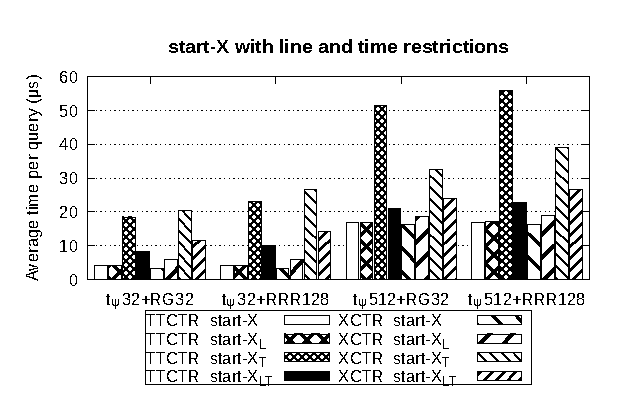
\includegraphics[width=\linewidth]{experiments/start.eps}
    \vspace{-12pt}
    \caption{}
    \vspace{-12pt}
    \end{subfigure}%
    \begin{subfigure}{0.5\linewidth}
    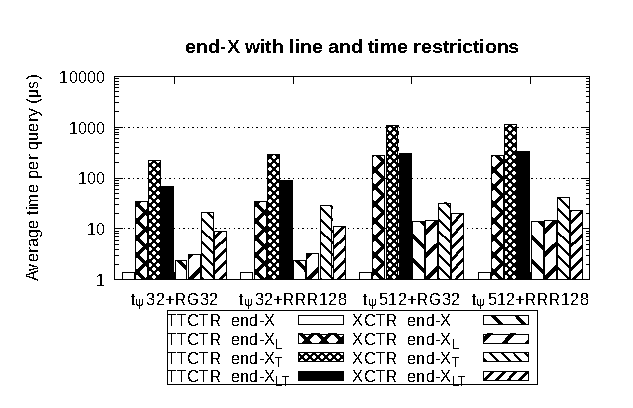
\includegraphics[width=\linewidth]{experiments/end.eps}
    \vspace{-12pt}
    \caption{}
    \vspace{-12pt}
    \end{subfigure}
    \caption{Comparison of \texttt{\startX$_{LT}$} (a) and \texttt{\endX$_{LT}$} (b) queries, with all variants. Note the logarithmic scale for the y axis in (b).}
    \label{fig:start}
    \end{figure}
    
    Recall that restricting both the line and time is always cheaper than only restricting the time, as for the latter more operations need to be performed to filter out every line. This explains why $T$ queries are always slower than $LT$ queries. This is true for both representations, with any configuration and query.
    
    \medskip
    We can see more examples of this difference in performance between our two representations with the \texttt{from\_X\_to\_Y} queries in Figure~\ref{fig:xy0}, whenever the end lines or times are restricted. Additionally, we can observe yet again how using the most sparse sampling of $\Psi$ affects much more the performance of \gls{ttctr}~than that of \gls{xctr}, with the performance of \texttt{from\_X$_{T}$\_to\_Y} consistent with the \texttt{\startX$_T$} shown in Figure~\ref{fig:start}a.
    
    \begin{figure}[ht]
    \begin{subfigure}{0.5\linewidth}
    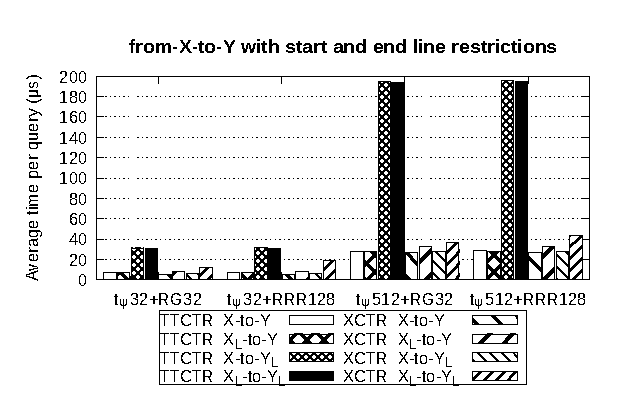
\includegraphics[width=\linewidth]{experiments/xy0.eps}
    \vspace{-12pt}
    \caption{}
    \vspace{-12pt}
    \end{subfigure}%
    \begin{subfigure}{0.5\linewidth}
    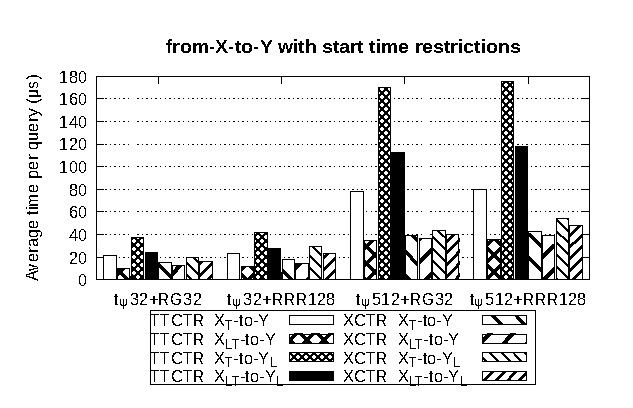
\includegraphics[width=\linewidth]{experiments/xy1.eps}
    \vspace{-12pt}
    \caption{}
    \vspace{-12pt}
    \end{subfigure}
    \caption{Comparison of \texttt{from\_X$_{LT}$\_to\_Y$_{LT}$} queries, variating line (a) and starting time (b) restrictions.}
    \label{fig:xy0}
    \end{figure}
    
    The performance of both representations can sometimes improve  when more selective restrictions are added, where the execution is cut short when no matching trips are found, before evaluating further restrictions. For this reason, the average times for \texttt{from\_X$_{T}$\_to\_Y$_{L}$} and \texttt{from\_X$_{LT}$\_to\_Y$_{L}$} are faster than those of \texttt{from\_X\_to\_Y$_{L}$} and \texttt{from\_X$_{L}$\_to\_Y$_{L}$}.
    
    When restricting to the end time, \gls{xctr}~consistently outperforms \gls{ttctr}, as shown in Figure~\ref{fig:xy2}. This was expected considering the large number of times that the \gls{csa} from \gls{ttctr}~needs to be queried, yielding results similar to those from Figure~\ref{fig:start}b where the end time is also restricted.
    
    \begin{figure}[ht]
    \begin{subfigure}{0.5\linewidth}
    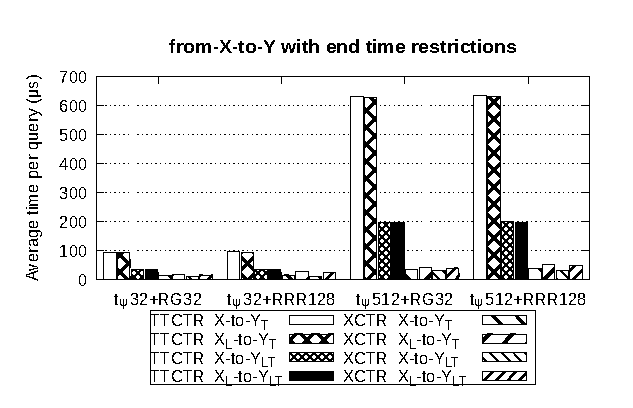
\includegraphics[width=\linewidth]{experiments/xy2.eps}
    \vspace{-12pt}
    \caption{}
    \vspace{-12pt}
    \end{subfigure}%
    \begin{subfigure}{0.5\linewidth}
    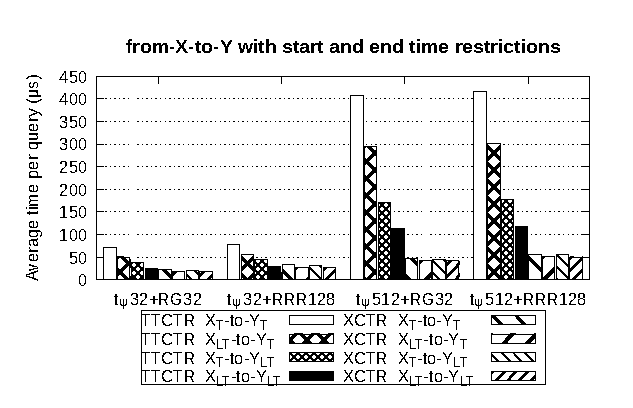
\includegraphics[width=\linewidth]{experiments/xy3.eps}
    \vspace{-12pt}
    \caption{}
    \vspace{-12pt}
    \end{subfigure}
    \caption{Comparison of \texttt{from\_X$_{LT}$\_to\_Y$_{LT}$} queries, variating line (a) and starting time (b) restrictions with a fixed ending time restriction.}
    \label{fig:xy2}
    \end{figure}
    
    The high selectivity of time restrictions explain why \gls{ttctr}~ becomes more competitive with the most restrictive queries of Figure~\ref{fig:xy2}b. However, its query time still increases several times when the \gls{csa} is highly compressed.
    
    \medskip
    The only query for which \gls{ttctr}~is clearly preferred over \gls{xctr}~is \boardX, with any restriction, as it can be seen in Figure~\ref{fig:board}a. Both for \boardX~and~\boardX$_{L}$, \gls{ttctr}~takes on average less than one microsecond per query, as the only operations needed are two constant time $\select_1$ over the bitvector $D$ from the \gls{csa}, while \gls{xctr}~needs to subtract the occurrences of $X\$$ (as those are alighting stops, not boarding), for which $\Psi$ must be accessed. This advantage is carried on the queries with time restrictions as well.
    
    \begin{figure}[ht]
    \begin{subfigure}{0.5\linewidth}
    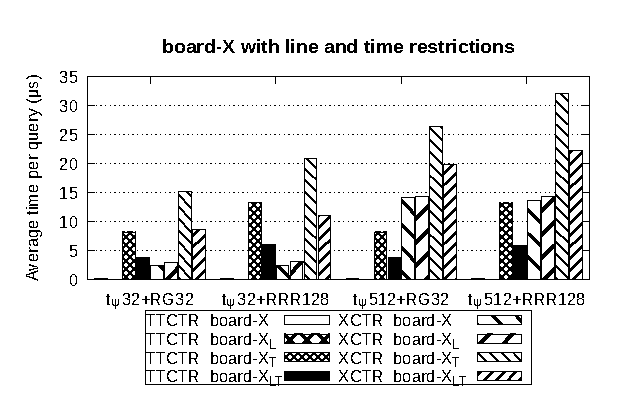
\includegraphics[width=\linewidth]{experiments/board.eps}
    \vspace{-12pt}
    \caption{}
    \vspace{-12pt}
    \end{subfigure}%
    \begin{subfigure}{0.5\linewidth}
    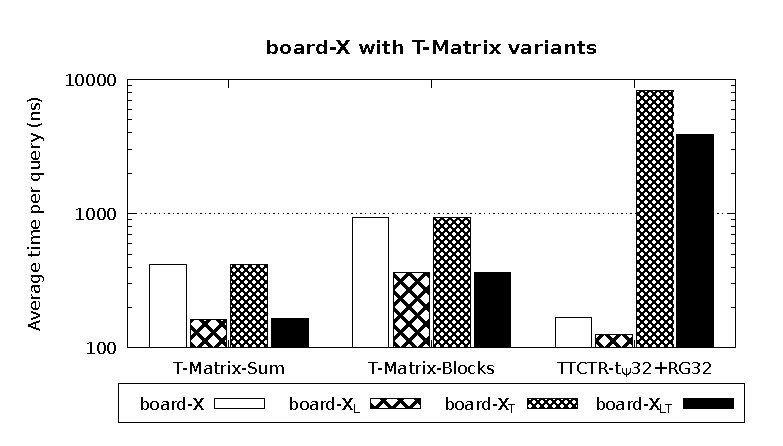
\includegraphics[width=\linewidth]{experiments/board_t.eps}
    \vspace{-12pt}
    \caption{}
    \vspace{-12pt}
    \end{subfigure}
    \caption{Comparison of \texttt{\boardX$_{LT}$} queries, with all variants (a) and also with all variants of \acrshort{tm}~(b). Note the logarithmic scale in (b), as well as the measurements in nanoseconds.}
    \label{fig:board}
    \end{figure}
    
    \medskip
    When comparing the best performing configuration of \gls{ttctr}~with the different variants of \gls{tm}~discussed in Section~\ref{sec:newctr:str:tm}, we can observe wildly different results in Figure~\ref{fig:board}b depending on the variant of the \boardX~query used. The biggest difference is observed when comparing queries that filter by time, which use the \gls{wm} in \gls{ttctr}, while any variant of \gls{tm}~solves it in a small number of $O(1)$ operations. Another evident difference occurs within each \gls{tm}~variant, where the queries that are restricted to a single line are significantly faster than those that consider every line, as the latter must query a different matrix for every line where the stop occurs in. It was also expected to see the compressed variant \texttt{Blocks} to perform slower than the uncompressed \texttt{Sum}, as the two former store relative values that must be resolved, increasing the number of memory accesses, although still by a constant factor. This also hints for a reason why the queries \boardX and \boardX$_{L}$ seem to be slightly faster in \gls{ttctr}~than any of the \gls{tm}, as a higher number of accesses over larger memory regions in \gls{tm}~makes cache misses more frequent. Nevertheless, the difference is very small, within the same microsecond.
    
    Obviously, \gls{tm}~may be used to solve other queries more efficiently than \gls{ttctr}~or \gls{xctr}. We did not find it interesting to report the run times for those queries as they are mostly equal to those shown in Figure~\ref{fig:board}b, due to being resolved with the same CPU operations. Refer to the complexities in Table~\ref{tab:queries} to obtain an accurate estimate of the time that it would take \gls{tm}~to solve each of the supported queries.
